\documentclass[10pt]{article}

\usepackage[top=1in, bottom=1in, left=.5in]{geometry}

\title{EXTERNAL INTERFACE REQUIREMENTS, PERFORMANCE REQUIREMENTS, DESIGN CONSTRAINTS AND DIAGRAMS FOR THE NAVIGATION MODULE}

\usepackage{graphicx}

\begin{document}
\maketitle
\tableofcontents


\section{External Performance requirements}
The system should have the standard fonts, icons, display the way points and the route in good color schemes to facilitate the navigation. The screen resolution should be very clear to enable the user navigate well. Standard buttons, functions, or navigation links that will appear on the screen, such as a help button, zoom in and out buttons, campus direction. System should have good Layout standards to support software localization for example catering for both Afrikaans and English languages. Voice recognition and instruction support just in case the user is visually impaired on the screen resolution is affected by sunshine well moving. The system shall by default consider user location as the starting point when finding the route and also be able to store and record his route.
\section{Performance requirements}
Navigation will require a stable wireless connection, GIS module services, places of interest information about the locations and database connection to fetch the venues, landmarks and buildings around campus. GIS will provide Services to gather, maintain, persist and provide information related to the world serviced by the system. It is about the creation and maintenance of a GIS Map of the campus.

Only android, web front end and iOS clients shall be able to use the application without the app draining much of their smartphones resources. 
\section{Design constraints}
The navigation should not require much bandwidth in displaying, recording and saving the route and connecting to the GIS maps. Preferably, a maximum of 5 seconds; this is intended to speed up the system response time to keep users interest high.   
The user must be notified when taking a different direction/route by the use of an arrow and the sound support. It should therefore have the ability to connect to various best routes from the user's location to the destination.
 \section{The Navigation Module}
 Once the user has selected the navigation page, s/he has to specify the location as the starting point and the destination provided they are all within campus otherwise the system displays a drop up list with corresponding locations as the user inputs the string variables. The best route with minimum number of way points(the simplest route) is displayed after the system has made calculations. Calculations depends on the GIS services and the areas selected by the user. The directions and distance to be covered are displayed However,the user select the popular route which is often used and saved.      
\subsection{user case for navigation }
system displays the navigation page\\
user selects the route\\
system calculates the route\\
user clicks the navigate button.
\subsubsection{}
 
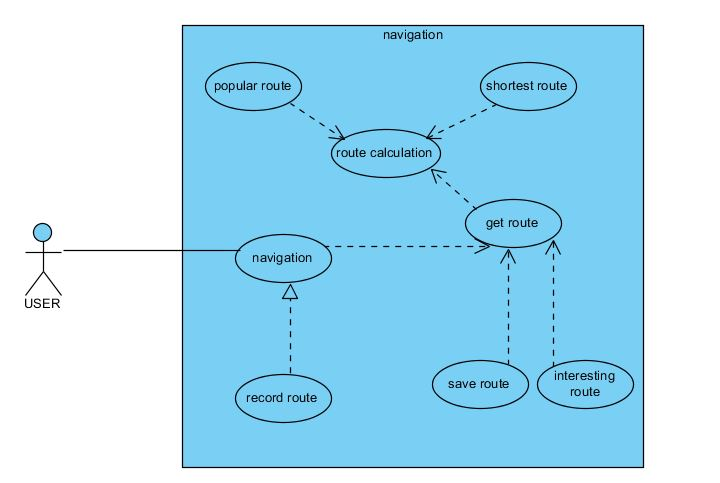
\includegraphics[width=8in, height=7in]{NUCD.JPG} 

\pagebreak
\subsection{activity diagram for navigation}

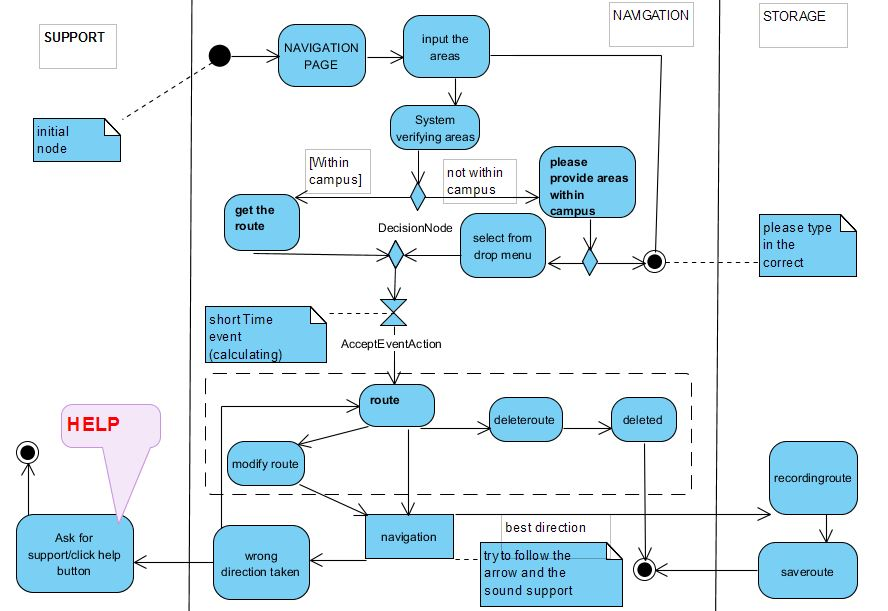
\includegraphics[width=8in, height=8in]{NAD.JPG} \\

\pagebreak
\subsection{class diagram for navigation}

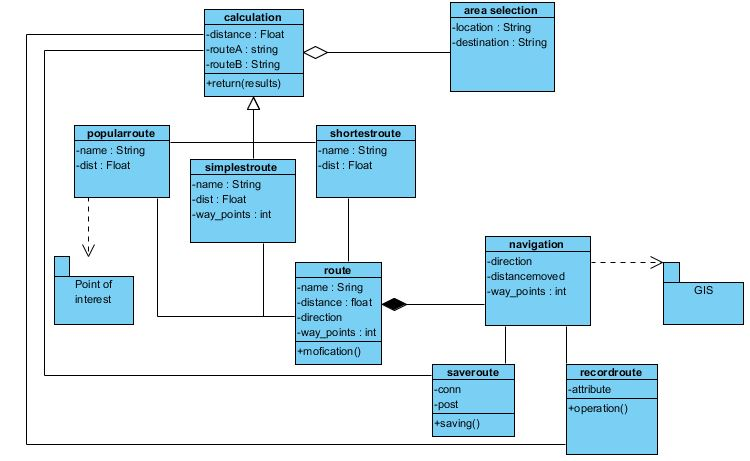
\includegraphics[width=8in, height=6in]{NCD.JPG} \\
\pagebreak
\subsection{Sequence diagram for navigation}

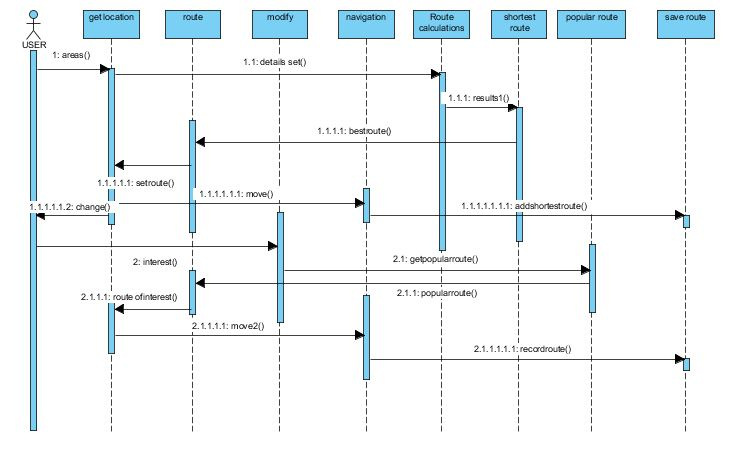
\includegraphics[width=8in, height=6in]{NSD.JPG} 


\end{document}